% !TeX program = lualatex
\documentclass[]{article}

\usepackage{caption,subcaption,graphicx,float,url,amsmath,amssymb,amsthm,tocloft,cancel,thmtools,gensymb,braket,tikz-feynman,mathtools}
\usepackage[toc,nonumberlist]{glossaries}
\usepackage{glossaries-extra}
\newcommand\numberthis{\addtocounter{equation}{1}\tag{\theequation}}

\newtheorem{thm}{Theorem}
\newtheorem{defn}[thm]{Definition}
\newtheorem{cor}[thm]{Corollary}
\newtheorem{lemma}[thm]{Lemma}
\graphicspath{{figs/}}
\widowpenalty10000
\clubpenalty10000
\setcounter{tocdepth}{2}
\tikzfeynmanset{compat=1.0.0}
%opening
\title{Theoretical Minimum\ Quantum Entanglement, Part 1}
\author{Simon Crase (compiler)\\simon@greenweaves.nz}

\begin{document}

\maketitle

\begin{abstract}
These are my notes from the Quantum Entanglement Part 1, lectures\cite{susskind2013entanglement}  from Leonard Susskind's Theoretical Minimum series\cite{susskind2007theoretical}.

Disclaimer: I have created these notes as an aide-m\'emoire for my own use; if you find them useful, you are welcome, but I'd appreciate hearing from you. They are not intended 
as a substitute for listening to the lectures. The intellectual property for all material derived from the lectures belongs, of course, to Professor Susskind; any mistakes, however, are my own.

The notes were created using TexStudio\cite{TexStudio}, which I recommend for compiling them to a PDF; the bibliography was created using JabRef\cite{Jabref}.

\end{abstract}

\tableofcontents
\listoffigures
\listoftables
\listoftheorems


\section{Introduction}


We, as animals, have inherited, through the process of evolution, certain intuitive ways of thinking about the physical world:
\begin{enumerate}
	\item Lioness pursuing antelope will stop as soon as relative velocity changes sign (physics calculation!);
	\item Neanderthal pushing rock from door of cave aims body to maximize component of force in the right direction.
\end{enumerate}

Everything in modern physics has to do with those things that are beyond these intuitions:
speeds approaching speed of light; 4 D; the electron; the uncertainty principle. Why would natural selecton have given us the intuition of the uncertainty principle? Intuitions for particles come from rocks.

This course will try to expose some of the weirdness of quantum mechanics, the weirdness of the logic quantum mechanics, the weirdness of how quantum information works. 

This course will cover:
\begin{enumerate}
	\item the basic logic of quantum mechanics;
	\item the basic logic of quantum information theory
	\item physics as information.
\end{enumerate}

Classical mechanics represents values as real numbers; QM often uses discrete values. Before we cover quantum bits we will look at classical bits, and we will use Dirac's notation\cite{susskind2014quantum} $\ket{0}$ or $\ket{1}$\cite{susskind2014quantum}. For an $n-bit$ \emph{classical} system, the number of configurations is $N_S=2^n$, so $n=\log_2(N_S)$.

We can generalize definition of number of bits of information: it doesn't have to be an integer. We can represent the state of a physical system, to specified precision, by a string of bits (quantize space, etc). Figure \ref{fig:state_transition} shows how the laws of physics can be represented as a state transition diagram.

\begin{figure}[H]
	\caption{The laws of physics can be represented as a state transition diagram. In quantum mechanics there is no fundamental difference between forward in time and backward in time.}\label{fig:state_transition}
	\begin{subfigure}[t]{0.45\textwidth}
		\caption{Reversible Laws}\label{fig:state_transition_reversible}
		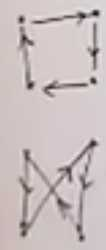
\includegraphics[width=0.8\textwidth]{et-1-1}
	\end{subfigure}
	\begin{subfigure}[t]{0.45\textwidth}
		\caption{An irreversible law}
		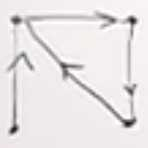
\includegraphics[width=0.8\textwidth]{et-1-2}
	\end{subfigure}
\end{figure}

All real systems are quantum mechanical. In this course we will try to answer the question why the quantum mechanics is suppressed in many systems we observe.

A Newtonian system is one that is in a definite state, and that evolves deterministically.

Second Law of Thermodynamics arises because we lose the ability to follow the evolution of a system in precise detail.

Review of vectors and matrices:
\begin{itemize}
	\item Row and column vectors as sequences of number;
	\item Inner products;
	\item Matrices--linear transformation of vectors.
\end{itemize}

We can represent a state by a "one hot" vector, and then represent the transitions of, say, Figure \ref{fig:state_transition_reversible}, by a matrix of ones and zeros.

\section{Review of Quantum Mechanics}

This section reviews material from \cite{susskind2013quantum}.
\subsection{Spin of a single electron}

Classical mechanics is based on classical logic. Classical logic means that the states are Boolean: a set of points, each representing a state, and all the logic is classical. Quantum mechanics depends on a completely different logic.

We start with a quantum bit of Qbit, such as the spin of an electron.

We need the concepts of \emph{preparing} a state, and \emph{detecting} a state.

Classically we can \emph{prepare} an electron to point in a particular direction by placing it in a magnetic field. The electron will precess before aligning: the stronger the field the faster it emits electromagnetic radiation and aligns.

To \emph{detect} we apply magnetic field, and measure radiation to see how much realignmnet was needed.

This is \emph{not} the way a real electron works.

A real electron behaves like this. No matter how we prepare the electron, when we turn on the magnetic field, either:
\begin{itemize}
	\item nothing happens; or
	\item it emits a single photon corresponding to the flip from down to up.
\end{itemize}
It is almost as if the electron has only two possible configurations. But what if we prepare it at $45^\circ$ or $90^\circ$? Still we get up or down. What if we measure in some other direction?

What if we prepare up, turn off field, and later measure? Up.

What if we prepare at $45^\circ$, turn off field, then measure up/down? Then there is a probability of emitting photon. Probability has memory of previous state. Once you measure, state is fixed.

In physics we have learned not to ask questions unless we can devise a way to measure the answer.


\subsection{Spins of two Electrons}

\begin{itemize}
	\item The state space is an abstract vector space.

	\item LS reviews vector spaces, bras and kets, and represents the electron pointing up as $\ket{+}$. The general representation for an electron is $a_+\ket{+}+a_-\ket{-}$, where $a_+^*a_+$ is the probability that we will find the electron in the up state. Normalized vectors represent physical states.
	
	\item We have to rewire ourselves to understand QM.

	\item Linear combinations of states correspond to preparation in different directions.
	
	\item The two notions of vector (spatial and abstract) are related, but not simply.
	
	\item Anything that we can measure (with a number) is an observable.
	
	\item If we knew the rules for calculating averages for all possible observables, we would also know how to compute the probability distribution.
	
	\item Hermitian matrices are the quantum equivalent of observables.
	
\end{itemize}


\section{Postulates of Quantum mechanics}
\subsection{Review (continued)}
This section continues the review of material from \cite{susskind2013quantum}.

\begin{itemize}
	\item Complex numbers
	\item The equation $e^{i\theta} = \cos{\theta} + i \sin{\theta}$ contains all of trigonometry.
\end{itemize}

\subsection{Postulates of Quantum mechanics}

\begin{enumerate}
	\item States are represented by normalized vectors.
	\item Observables are represented by Hermitian matrices.
	\item $\braket{a|M|a}$ - expectation
	\item Eigenvalues and Eigenvectors
\end{enumerate}


We need complex numbers to handle evolution with time.

Define:
\begin{align*}
	\sigma_3 =& \begin{bmatrix} 1&0\\
	0&-1
                \end{bmatrix}\\
            \sigma_2 =& \begin{bmatrix}
            	0 & -i\\
            	i & 0
            \end{bmatrix}\\
     \sigma_1 =& \begin{bmatrix} 0&1\\
         	1&0
     \end{bmatrix} 
\end{align*}
Then
\begin{align*}
		\sigma_3^2 =& 1\\
	\sigma_3^2 =& 1\\
	\sigma_1^2 =& 1
\end{align*}
and the eigenvalues are $\pm1$.


\begin{thm}[If $M$ is Hermitian and it has two different eigenvalues, then the eigenvectors are orthogonal.]
	\begin{align*}
		M =& M^\dagger \text{ and}\\
		M \ket{a} =& \lambda_a \ket{a}\text{ and}\\
		M \ket{b} =& \lambda_b \ket{b}\text{ and}\\
		\lambda_a \ne& \lambda_b \\
		\implies&\\
		\braket{a|b} =& 0
	\end{align*}
\end{thm}

https://youtu.be/CaTF4QZ94Fk?t=3707
\section{Quantum Entanglement}

\section{Quantum Entanglement}

\section{Quantum Entanglement}

\section{Quantum Entanglement}

\section{Quantum Entanglement}

\section{Quantum Entanglement}

\bibliographystyle{unsrt}
\addcontentsline{toc}{section}{Bibliography}
\raggedright
\bibliography{tm}

\end{document}